\chapter[\textsc{Yu. I. Manin~:} On Some Groups Related to Cubic Hyper-surfaces]{ON SOME GROUPS RELATED TO CUBIC HYPERSURFACES}\label{art13}

\begin{center}
{\em By}~~ Yu. I. Manin
\end{center}

\setcounter{pageoriginal}{254}
\section*{Introduction and motivation.}
\pageoriginale

\lhead[\thepage]{\textit{On Some Groups Related to Cubic Hyper-surfaces}}
\rhead[\textit{Yu. I. Manin}]{\thepage}

Let $V$ be a nonsingular cubic curve in a projective plane over a field $k$. If the set $V(k)$ of its $k$-points is nonempty, one may endow $V$ with a structure of an abelian variety over $k$, taking one of the points for identity. Then the group law on $V(k)$ may be easily described geometrically. The description is especially simple if identity is an inflexion point of $V$: then the sum of three points is identity if and only if they are collinear. It follows that the ternary relation $L(x,y,z)$ (``$x$, $y$, $z$ are collinear'') may be considered as the basic one for the theory of one-dimensional abelian varieties. This is the classical approach, which makes possible, for example, to give ``elementary'' proofs of Mordell-Weil theorem and Riemann conjecture for elliptic curves.

The ternary relation $L$ is defined not only for cubic curves but, say, for all geometrically irreducible cubic hypersurfaces in a projective\break space. However, this relation was scarcely utilized for studying of arithmetic and geometric properties of these varieties. One of the main reasons of it was that one could not relate $L$ to some standard algebraic structure: in fact, cubic hypersurfaces of dimension $\geq 2$ are definitely not group varieties.

In this talk we suggest and discuss two different ways to construct a group by means of the relation $L$.

The first way is to consider for any nonsingular point $x\in V(k)$ the birational automorphism $t_{x}:V\to V$, which in its existence domain is given by the relation $L(x,y,t_{x}(y))$. (In other words, $t_{x}$ is ``the reflection relatively to point $x$''). Then one may consider the group $B$, generated by automorphisms $t_{x}$ for all $x\in V(k)$ (or for some subset of points). If $\dim V=1$, this group $B$ is easily seen to be isomorphic to the canonical extension of $\bfZ_{2}$ by $V(k)$ with usual group law. In particular\pageoriginale one can reconstruct $V(k)$ from $B$. So one can hope that properties of the group $B$ are of some interest in the general case.

The second way to construct a group is to imitate the one-dimensio\-nal definition, but applying it to some classes of points of $V$ rather than the points themselves. Namely, consider a decomposition of $V(k)$ in disjoint subsets $V(k)=\cup C_{i}$, enjoying the following properties:
\begin{itemize}
\item[(a)] if $L(x,y,z)$, where $x\in C_{p}$, $y\in C_{q}$, $z\in C_{r}$, then any of classes $C_{p}$, $C_{q}$, $C_{r}$ is uniquely defined by the other two;

\item[(b)] on the set of classes $\{C_{i}\}$ there exists a structure of abelian group $\Gamma$ of {\em period two} such that the relation ``sum of three classes is equal to zero'' coincides with the relation, induced by $L$ on this set.
\end{itemize}

(All this simply means that one can add two classes, drawing a line through its representatives and then taking the class of the third point of intersection of this line with $V$. In fact, one must be a little bit more careful to avoid lines lying in $V$: c.f. the statement of Theorem \ref{art13-thm3} below.)

An example of such decomposition in case $\dim V=1$ is given by the family of cosets $V(k)/2V(k)$. So the groups constructed by this procedure are similar to ``weak Mordell-Weil groups''. F. Ch\^atelet has discovered nontrivial groups of this kind for certain singular cubic surfaces \cite{art13-key1}.

We shall describe now briefly our main results. The first section below contains complete definitions and statements, the second gives some ideas of proof.

The group $B$ is studied in some detail for nonsingular cubic surfaces. In particular, we give a complete system of relations between maps $t_{x}$ for $x$, not lying on the union of $27$ lines of $V$. Besides, we prove, that for $k$-minimal surfaces such $t_{x}$ together with the group of projective transformations of $V$ generate the whole group of birational $k$-automorphisms of $V$ (Theorems \ref{art13-thm1} and \ref{art13-thm2}).

The main result on the group $\Gamma$ of classes of points of $V(k)$ is proved for all dimensions and states the existence of the unique ``finest''\pageoriginale decomposition or ``biggest'' group $\Gamma$. In fact, we consider such decompositions not only of the total set $V(k)$, but of any subset of it fulfilling some natural conditions. It happens then that, say, the identity class of any such decomposition may be decomposed again and so on. So one can construct for any $V$ a sequence of $2$-groups $\Gamma_{n}$ which for $\dim V=1$ is given by $\Gamma_{n}=2^{n}V(k)/2^{n+1}V(k)$ (Theorem \ref{art13-thm3}).

The last Theorem \ref{art13-thm4} shows a connection between groups $B$ and $\Gamma$.

\section*{Main statements.}

Let $V$ be a nonsingular cubic surface in $\bfP^{3}$, defined over a field $k$. All points we consider are geometric $K$-points for subfields $K$ of an algebraic closure $\overline{k}$ of $k$.

A point $x\in V(\overline{k})$ is called {\em nonspecial}, if it does not belong to the union of 27 lines on $V\otimes \overline{k}$.

A pair of points $(x,y)\in V(\overline{k})\times V(\overline{k})$ is called {\em nonspecial}, if points $x$, $y$ are distinct and nonspecial and if the line in $\bfP^{3}$, containing $x$, $y$, is not tangent to $V$ and is disjoint with any line of $V\otimes\overline{k}$.

For any point $x\in V(k)$ the birational $k$-automorphism $t_{x}:V\to V$ is defined (c.f. Introduction). If the point $t_{x}(y)$ is defined, we shall sometimes denote it $x\circ y$. If $x\circ y$ and $y\circ x$ are both defined, then $x\circ y=y\circ x$.

\medskip
\noindent
{\bf Theorem \thnum{1}.\label{art13-thm1}}
{\em Let $W$ be the group of projective automorphisms of $V\otimes \overline{k}$ over $\overline{k}$ and $B$ the group of birational automorphisms generated by the reflections $t_{x}$ relative to the nonspecial points $x\in V(\overline{k})$.}

{\em Then the group, generated by $W$ and $B$, is the semidirect product of these subgroups with normal subgroup $B$ and the natural action}
$$
wt_{x}w^{-1}=t_{w(x)},\quad w\in W, \quad x\in V(\overline{k}).
$$

{\em Moreover, the complete system of relations between the generators $t_{x}$ of group $B$ is generated by}
\begin{equation*}
t^{2}_{x}=1;\quad (t_{x}t_{x\circ y}t_{y})^{2}=1\tag{1}\label{art13-eq1}
\end{equation*}
{\em for all nonspecial pairs $(x,y)$ of points of $V(\overline{k})$.}
\smallskip

In\pageoriginale particular, it follows from relations \eqref{art13-eq1}, that if $(x,y)$ is a non-special pair of points, defined and conjugate over a quadratic extension $K/k$, then the $K$-automorphism $t_{x}t_{x\circ y}t_{y}$ of $V\otimes K$ is obtained by the ground field extension from some $k$-automorphism of $V$ which we shall denote $s_{x,y}$.

\medskip
\noindent
{\bf Theorem \thnum{2}.\label{art13-thm2}}
{\em Suppose moreover that $k$ is perfect and the surface $V$ is $k$-minimal (i.e. any birational $k$-morphism $V\to V'$ is an isomorphism). Then the group of birational $k$-automorphisms of $V$ is generated by the subgroup of its projective automorphisms and by elements $t_{x}$, $s_{x,y}$ for all nonspecial points $x\in V(k)$ and for all nonspecial pairs of points $(x,y)$, defined and conjugate over some quadratic extension of $k$.}
\smallskip

We note that in the paper \cite{art13-key2} the following statement was proved: {\em two minimal cubic surfaces are birationally equivalent over $k$ if and only if they are} ({\em projectively}) {\em isomorphic}. So Theorems \ref{art13-thm1} and \ref{art13-thm2} give us a fairly complete description of the category of such surfaces and birational applications. Note also an analogy with the category of one-dimensional abelian varieties. It suggests the desirability to investigate also rational applications of finite degree (``isogenies'').

To compare the two-dimensional case with one-dimensional one note that if $\dim V=1$, then
\begin{equation*}
t^{2}_{x}=1,\quad (t_{x}t_{y}t_{z})^{2}=1\tag{2}\label{art13-eq2}
\end{equation*}
for {\em all triples} $(x,y,z)$ of points of $V$. But even this is not a complete system of relations: there exist relations, depending on the structure of $k$ and on the particular nature of some points. Thus in dimension 2 the properties of group $B$ are less subtle.

The statement of Theorem \ref{art13-thm1} without essential changes should be valid for all dimensions $\geq 2$.

Now we shall state the main notions necessary to define the groups $\Gamma$.

Let $V$ be a geometrically irreducible cubic hypersurface over a field $k$. Let $C\subset V(k)$ be a Zariski-dense set of points of $V$. We say that a subset $C'\subset C$ consists of {\em almost all} points of $C$, if $C'$ contains the intersection of $C$ with a Zariski-dense open subset of $V$.

The\pageoriginale following definition describes a class of sets $C$, for which we can construct ``group decompositions''.

\begin{defi*}
$C\subset V(k)$ is called an admissible set, if the following two conditions are fulfilled.
\begin{itemize}
\item[\rm(a)] $C$ is Zariski-dense and consists only of nonsingular points of $V$.

\item[\rm(b)] Let $x\in C$. Then for almost all points $y\in C$ the point $t_{x}(y)$ is defined and belongs to $C$.
\end{itemize}
\end{defi*}

The following sets, if they are dense, are admissible:
\begin{enumerate}
\item the set of all nonsingular points of $V$;

\item the set of hyperbolic points of a nonsingular cubic surface over $\bfR$, if it is a connected component of $V(\bfR)$;

\item the minimal set, containing a given system of points and closed under the relation $L$.
\end{enumerate}

\medskip
\noindent
{\bf Theorem \thnum{3}.\label{art13-thm3}}
{\em Let $C\subset V(k)$ be an admissible set. Let $\Gamma(C)$ be the abelian group, generated by the family of symbols $C(x)$ for all $x\in C$, subject to following relations :}
\begin{equation*}
2C(x)=0,\quad C(x)+C(y)+C(z)=0\tag{3}\label{art13-eq3}
\end{equation*}
{\em for all triples of different points $x$, $y$, $z\in C$, lying on a line not belonging to $V$. Then the map of sets}
$$
C\to \Gamma(C):x\to C(x)
$$
{\em is surjective. Thus the group $\Gamma(C)$ is isomorphic to a group of classes of $C$ under certain equivalence relation, with the composition law ``drawing a line through two points''.}

{\em Moreover, the union of classes, corresponding to any subgroup of $\Gamma(C)$, is an admissible set.}
\smallskip

From this theorem it is clear that any different ``group decomposition'' of $\Gamma(C)$ (c.f. Introduction) can be obtained from the one constructed by collecting together cosets of some subgroup of $\Gamma(C)$. 

As was stated, for $\dim V=1$ and $C=V(k)$ we have $\Gamma(C)=V(k)/2V(k)$. A certain modification of this result remains valid in the dimension two.

\medskip
\noindent
{\bf Theorem \thnum{3}.\label{art13-thm4}}
{\em Let\pageoriginale $C$ be an admissible subset of nonspecial points of a nonsingular cubic surface $V$. Let $B(C)$ be the group of birational automorphisms of $V$, generated by $t_{x}$, $x\in C$, and $B_{0}(C)\subset B(C)$ the normal subgroup generated by $s_{x,y}$ for all nonspecial pairs $(x,y)\in C\times C$. Then}
$$
\Gamma(C)\simeq B(C)/B_{0}(C).
$$
\smallskip

This is an easy consequence of the Theorem \ref{art13-thm1} and so probably generalizes to all dimensions $\geq 2$.

Our knowledge of groups $\Gamma(C)$ is very poor. Unlike groups $B$ they depend on the constant field $k$ in a subtle way. For example, if $C$ consists of all nonsingular points of $V$ in an algebraically closed field, the $\Gamma(C)=\{0\}$ (as is the one-dimensional case: the group of points of an abelian variety is divisible).

On the other hand, I can construct examples of nonsingular cubic surfaces $V$ over number fields $k$ such that the group $C(V(k))$ has arbitrarily many generators. I do not know whether it can be infinite. Perhaps for a reasonable class of varieties a kind of ``weak Mordell-Weil theorem'' is true.

We wish to formulate some more problems which arise naturally in connection with our construction. Beginning with some admissible set $C_{0}$, denote by $C_{1}\subset C_{0}$ the identity class of $\Gamma(C_{0})$. As $C_{1}$ is admisible, we can construct the identity class of $\Gamma(C_{0})$, and so on. Let $C_{i+1}$ be the identity class of $\Gamma(C_{i})$; we get a sequence of sets of points $C_{0}\supset C_{1}\supset C_{2}\supset \cdots$ and of groups $\Gamma(C_{i})$.

Let $k$ be a number field and $C_{0}=V(k)$. Does the sequence $\{C_{i}\}$ stabilize? What is the intersection $\cap C_{i}$? (In the one-dimensional case it consists of points of odd order). Is it possible to ``put together'' all of groups $\Gamma(C_{i})$ by constructing an universal group and say, a normal series of it, with factors $\Gamma(C_{i})$ ?

Theorem \ref{art13-thm4} shows a certain approach to the last question. In fact, $\Gamma(C_{i})=B(C_{i})/B_{0}(C_{i})$, where
$$
B(C_{0})\supset\cdots\supset B(C_{i})\supset B_{0}(C_{i})\supset B(C_{i+1})\supset \cdots
$$
But the ``gaps'' $B_{0}(C_{i})\supset B(C_{i+1})$ are probably nontrivial.

One\pageoriginale of the serious obstacles to studying $\Gamma(V(k))$ is the lack of a manageable criterion for a point to be in the identity class. More generally, one would like to have a substitute for the basic homomorphism
$$
\delta : V(k)/2V(k)\to H^{1}(k_{,2}V(k)),
$$
of one-dimensional case.

\subsection*{Ideas of proofs.}
Theorem \ref{art13-thm1} is proved by a refinement of methods, developed in the section 5 of \cite{art13-key2}, where a complete proof of Theorem \ref{art13-thm2} is given.

Let $V$ be a (nonsingular) projective $k$-surface. Let $Z(V)=\varinjlim\break \Pic (V')$, where the system of groups $\Pic$ is indexed by the set of birational $\overline{k}$-morphisms $V'\to V\otimes \overline{k}$ with natural dominance relation. The group $Z(V)$ is endowed with the following structures all of which are induced from ``finite levels''.
\begin{enumerate}
\item $Z(V)$ is a $G$-module, where $G=\Gal (\overline{k}/k)$;

\item there is a $G$-invariant pairing ``intersection index'' $Z(V)\times Z(V)\to \bfZ$;

\item there is a $G$-invariant augmentation $Z(V)\to \bfZ$ : ``intersection index with the canonical class'';

\item the cone of positive elements $Z^{+}(V)$;

\item the cone $Z^{++}(V)$, dual to $Z^{+}(V)$ relative to the pairing.
\end{enumerate}

\eject

Now for any $k$-birational map $f:V'\to V$ an isomorphism $f^{*}:Z(V)\to Z(V')$ is defined, preserving all of the structures above, and $(fg)^{*}=f^{*}g^{*}$. In particular, the group of birational $k$-automorphisms of $V$ is represented in the group $Z(V)$.

\vskip .05cm

To use this representation effectively, one must look at the group $Z(V)$ differently.

\vskip .05cm

Construct a prescheme $E(V)=(\cup V')/R$, the sum of all $V'$, $k$-birationally mapped onto $V\otimes\overline{k}$, by the equivalence relation $R$, which\pageoriginale patches together the biggest open subsets of $V'$ and $V''$ isomorphic under the natural birational application $V'\longleftrightarrow V''$.

\vskip .05cm

To understand better the architecture of $E(V)$, look at the simplest morphism $V'\to V$, contracting a line $l$ onto a point $x$. Patching $V'$ and $V$ by identifying $V'\backslash l$ with $V'\backslash x$, we get a little bit of $E(V)$. If $k=\bfC$, $l$ is the Riemann sphere; so the result of patching may be viewed as $V$ complemented by a ``bubble'' blown up from the point $x\in V$. To get the whole $E(V)$ one must blow up bubbles from all points of $V$, then from all points of these bubbles, and so on. So I suggest to call this $E(V)$ ``the bubble space'' associated to $V$.

\vskip .05cm

Now, this bubble space is connected with $Z(V)$ as follows. Each point of $Z(V)(\overline{k})$ defines its bubble to which in turn corresponds a certain element of $Z(V)$. So there is the natural homomorphism
$$
\Pic (V\otimes \overline{k})\oplus C^{0}(E(V))\to Z(V)
$$
where $C^{0}(V)$ is the free abelian group, generated by all $\overline{k}$-points of $V$.

\vskip .05cm

In fact it is an isomorphism. The structures on $Z(V)$, defined earlier, have a rather detailed description in this new setting. On the other hand this presentation of $Z(V)$ is well fit for calculations giving a nice ``geometric'' set of generators for $Z(V)$.

\vskip .05cm

We omit these calculations which are rather long, especially those in the proof of Theorem \ref{art13-thm1}. Note only some similarity with the description of all relations in Coxeter groups generated by reflections in an Euclidian space.

\vskip .05cm

The proof of Theorem \ref{art13-thm3} is much more elementary. To prove the surjectivity of $C\to \Gamma(C)$ it is sufficient to find for any $x$, $y\in C$ a third point $z\in C$ such that $C(x)+C(y)=C(z)$. We say that points $x$, $y\in C$ are {\em in general position}, if the line, containing them, is not tangent to $V$ (and in particular does not belong to $V$) and the third intersection point of this line with $V$ belongs to $C$. Then, by definition, $C(x)+C(y)=C(z)$. So one must consider the case, when $x$, $y$ are not in general position. One can find such points\pageoriginale $u$, $v\in C$, that the following pairs of points are in general position:
$$
(x,u);\quad (t_{u}(x),v); (t_{v}t_{u}(x),u\circ v);\quad (t_{u\circ v}t_{v}t_{u}(x),y).
$$
\begin{figure}[H]
\centering
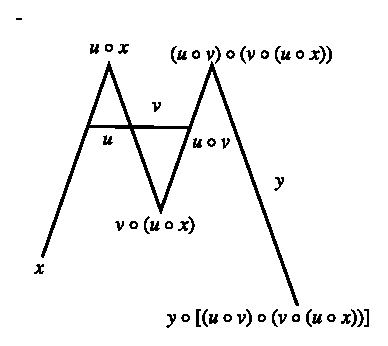
\includegraphics{src/chap13/fig1.eps}
\end{figure}

\vskip .05cm

So we are done:
$$
C(x)+C(y)=C(x)+C(u)+C(v)+C(u\circ v)+C(y)=C(y\circ (t_{u\circ v}t_{v}t_{u}x)).
$$

To find points $(u,v)$ one may work in $V(k)$, because $C$ is dense, and then one sees that such points exist on a plane section through $(x,y)$.

\vskip .05cm

The same argument shows the density and consequently the admissibility of a subgroup of $\Gamma(C)$.

\newpage

\begin{thebibliography}{99}
\bibitem{art13-key1} \textsc{F. Ch\^atelet :} Points rationnels sur certaines courbes et surfaces cubiques, {\em Enseignement mathematique,} 5, 1959, 153-170.

\bibitem{art13-key2} \textsc{Yu. I. Manin :} Rational surfaces over perfect fields, II, {\em Matematiceskii Sbornik},. 72, N2 (1967), pp. 161-192 (in Russian).
\end{thebibliography}

\bigskip
\noindent
{\small Mat. Inst. AN SSSR}

\noindent
{\small Moscow}



